% Options for packages loaded elsewhere
\PassOptionsToPackage{unicode}{hyperref}
\PassOptionsToPackage{hyphens}{url}
%
\documentclass[
]{article}
\usepackage{amsmath,amssymb}
\usepackage{lmodern}
\usepackage{iftex}
\ifPDFTeX
  \usepackage[T1]{fontenc}
  \usepackage[utf8]{inputenc}
  \usepackage{textcomp} % provide euro and other symbols
\else % if luatex or xetex
  \usepackage{unicode-math}
  \defaultfontfeatures{Scale=MatchLowercase}
  \defaultfontfeatures[\rmfamily]{Ligatures=TeX,Scale=1}
\fi
% Use upquote if available, for straight quotes in verbatim environments
\IfFileExists{upquote.sty}{\usepackage{upquote}}{}
\IfFileExists{microtype.sty}{% use microtype if available
  \usepackage[]{microtype}
  \UseMicrotypeSet[protrusion]{basicmath} % disable protrusion for tt fonts
}{}
\makeatletter
\@ifundefined{KOMAClassName}{% if non-KOMA class
  \IfFileExists{parskip.sty}{%
    \usepackage{parskip}
  }{% else
    \setlength{\parindent}{0pt}
    \setlength{\parskip}{6pt plus 2pt minus 1pt}}
}{% if KOMA class
  \KOMAoptions{parskip=half}}
\makeatother
\usepackage{xcolor}
\usepackage[margin=1in]{geometry}
\usepackage{color}
\usepackage{fancyvrb}
\newcommand{\VerbBar}{|}
\newcommand{\VERB}{\Verb[commandchars=\\\{\}]}
\DefineVerbatimEnvironment{Highlighting}{Verbatim}{commandchars=\\\{\}}
% Add ',fontsize=\small' for more characters per line
\usepackage{framed}
\definecolor{shadecolor}{RGB}{248,248,248}
\newenvironment{Shaded}{\begin{snugshade}}{\end{snugshade}}
\newcommand{\AlertTok}[1]{\textcolor[rgb]{0.94,0.16,0.16}{#1}}
\newcommand{\AnnotationTok}[1]{\textcolor[rgb]{0.56,0.35,0.01}{\textbf{\textit{#1}}}}
\newcommand{\AttributeTok}[1]{\textcolor[rgb]{0.77,0.63,0.00}{#1}}
\newcommand{\BaseNTok}[1]{\textcolor[rgb]{0.00,0.00,0.81}{#1}}
\newcommand{\BuiltInTok}[1]{#1}
\newcommand{\CharTok}[1]{\textcolor[rgb]{0.31,0.60,0.02}{#1}}
\newcommand{\CommentTok}[1]{\textcolor[rgb]{0.56,0.35,0.01}{\textit{#1}}}
\newcommand{\CommentVarTok}[1]{\textcolor[rgb]{0.56,0.35,0.01}{\textbf{\textit{#1}}}}
\newcommand{\ConstantTok}[1]{\textcolor[rgb]{0.00,0.00,0.00}{#1}}
\newcommand{\ControlFlowTok}[1]{\textcolor[rgb]{0.13,0.29,0.53}{\textbf{#1}}}
\newcommand{\DataTypeTok}[1]{\textcolor[rgb]{0.13,0.29,0.53}{#1}}
\newcommand{\DecValTok}[1]{\textcolor[rgb]{0.00,0.00,0.81}{#1}}
\newcommand{\DocumentationTok}[1]{\textcolor[rgb]{0.56,0.35,0.01}{\textbf{\textit{#1}}}}
\newcommand{\ErrorTok}[1]{\textcolor[rgb]{0.64,0.00,0.00}{\textbf{#1}}}
\newcommand{\ExtensionTok}[1]{#1}
\newcommand{\FloatTok}[1]{\textcolor[rgb]{0.00,0.00,0.81}{#1}}
\newcommand{\FunctionTok}[1]{\textcolor[rgb]{0.00,0.00,0.00}{#1}}
\newcommand{\ImportTok}[1]{#1}
\newcommand{\InformationTok}[1]{\textcolor[rgb]{0.56,0.35,0.01}{\textbf{\textit{#1}}}}
\newcommand{\KeywordTok}[1]{\textcolor[rgb]{0.13,0.29,0.53}{\textbf{#1}}}
\newcommand{\NormalTok}[1]{#1}
\newcommand{\OperatorTok}[1]{\textcolor[rgb]{0.81,0.36,0.00}{\textbf{#1}}}
\newcommand{\OtherTok}[1]{\textcolor[rgb]{0.56,0.35,0.01}{#1}}
\newcommand{\PreprocessorTok}[1]{\textcolor[rgb]{0.56,0.35,0.01}{\textit{#1}}}
\newcommand{\RegionMarkerTok}[1]{#1}
\newcommand{\SpecialCharTok}[1]{\textcolor[rgb]{0.00,0.00,0.00}{#1}}
\newcommand{\SpecialStringTok}[1]{\textcolor[rgb]{0.31,0.60,0.02}{#1}}
\newcommand{\StringTok}[1]{\textcolor[rgb]{0.31,0.60,0.02}{#1}}
\newcommand{\VariableTok}[1]{\textcolor[rgb]{0.00,0.00,0.00}{#1}}
\newcommand{\VerbatimStringTok}[1]{\textcolor[rgb]{0.31,0.60,0.02}{#1}}
\newcommand{\WarningTok}[1]{\textcolor[rgb]{0.56,0.35,0.01}{\textbf{\textit{#1}}}}
\usepackage{longtable,booktabs,array}
\usepackage{calc} % for calculating minipage widths
% Correct order of tables after \paragraph or \subparagraph
\usepackage{etoolbox}
\makeatletter
\patchcmd\longtable{\par}{\if@noskipsec\mbox{}\fi\par}{}{}
\makeatother
% Allow footnotes in longtable head/foot
\IfFileExists{footnotehyper.sty}{\usepackage{footnotehyper}}{\usepackage{footnote}}
\makesavenoteenv{longtable}
\usepackage{graphicx}
\makeatletter
\def\maxwidth{\ifdim\Gin@nat@width>\linewidth\linewidth\else\Gin@nat@width\fi}
\def\maxheight{\ifdim\Gin@nat@height>\textheight\textheight\else\Gin@nat@height\fi}
\makeatother
% Scale images if necessary, so that they will not overflow the page
% margins by default, and it is still possible to overwrite the defaults
% using explicit options in \includegraphics[width, height, ...]{}
\setkeys{Gin}{width=\maxwidth,height=\maxheight,keepaspectratio}
% Set default figure placement to htbp
\makeatletter
\def\fps@figure{htbp}
\makeatother
\setlength{\emergencystretch}{3em} % prevent overfull lines
\providecommand{\tightlist}{%
  \setlength{\itemsep}{0pt}\setlength{\parskip}{0pt}}
\setcounter{secnumdepth}{-\maxdimen} % remove section numbering
\ifLuaTeX
  \usepackage{selnolig}  % disable illegal ligatures
\fi
\IfFileExists{bookmark.sty}{\usepackage{bookmark}}{\usepackage{hyperref}}
\IfFileExists{xurl.sty}{\usepackage{xurl}}{} % add URL line breaks if available
\urlstyle{same} % disable monospaced font for URLs
\hypersetup{
  pdftitle={DP Second Laboratory},
  pdfauthor={Teresa Ricciardi; Albert Bertran},
  hidelinks,
  pdfcreator={LaTeX via pandoc}}

\title{DP Second Laboratory}
\author{Teresa Ricciardi \and Albert Bertran}
\date{2023-04-10}

\begin{document}
\maketitle

\begin{Shaded}
\begin{Highlighting}[]
\FunctionTok{library}\NormalTok{(sdcMicro)}
\FunctionTok{data}\NormalTok{(}\StringTok{"free1"}\NormalTok{) }\CommentTok{\# loads the dataset}
\end{Highlighting}
\end{Shaded}

\hypertarget{pram-post-randomization-method}{%
\subsection{1.PRAM (Post Randomization
Method)}\label{pram-post-randomization-method}}

\hypertarget{a-use-table-to-obtain-the-frequencies-for-each-category-of-the-marstat-variable-of-the-free1-dataset.-define-your-own-p-matrix-remember-the-sum-of-the-rows-must-be-1-and-calculate-the-theoretical-expected-frequency-for-each-category-after-praming-the-marstat-variable.-are-the-expected-values-of-the-frequencies-after-praming-similar-to-the-original-ones-first-we-create-a-newdataset-from-the-free1-dataset-and-we-check-the-different-values-marstat-has.}{%
\subsubsection{a) Use table() to obtain the frequencies for each
category of the MARSTAT variable of the free1 dataset. Define your own P
matrix (remember the sum of the rows must be 1) and calculate the
theoretical expected frequency for each category after ``praming'' the
MARSTAT variable. Are the expected values of the frequencies after
``praming'' similar to the original ones? First, we create a newdataset
from the ``free1'' dataset and we check the different values MARSTAT
has.}\label{a-use-table-to-obtain-the-frequencies-for-each-category-of-the-marstat-variable-of-the-free1-dataset.-define-your-own-p-matrix-remember-the-sum-of-the-rows-must-be-1-and-calculate-the-theoretical-expected-frequency-for-each-category-after-praming-the-marstat-variable.-are-the-expected-values-of-the-frequencies-after-praming-similar-to-the-original-ones-first-we-create-a-newdataset-from-the-free1-dataset-and-we-check-the-different-values-marstat-has.}}

\begin{Shaded}
\begin{Highlighting}[]
\NormalTok{newdataset}\OtherTok{\textless{}{-}}\NormalTok{free1}
\NormalTok{v }\OtherTok{\textless{}{-}} \FunctionTok{table}\NormalTok{(newdataset[,}\StringTok{"MARSTAT"}\NormalTok{])}
\NormalTok{v}
\end{Highlighting}
\end{Shaded}

\begin{verbatim}
## 
##    1    2    3    4 
## 2547  162  171 1120
\end{verbatim}

We now create a P matrix to use for pramming. The values used are just
the ones in the slides of the session.

\begin{Shaded}
\begin{Highlighting}[]
\NormalTok{mdat }\OtherTok{\textless{}{-}} \FunctionTok{matrix}\NormalTok{(}\FunctionTok{c}\NormalTok{(}\FloatTok{0.5}\NormalTok{,}\FloatTok{0.4}\NormalTok{,}\FloatTok{0.1}\NormalTok{,}\DecValTok{0}\NormalTok{,}
                 \FloatTok{0.1}\NormalTok{,}\FloatTok{0.6}\NormalTok{,}\FloatTok{0.2}\NormalTok{,}\FloatTok{0.1}\NormalTok{,}
                 \FloatTok{0.1}\NormalTok{,}\FloatTok{0.3}\NormalTok{,}\FloatTok{0.6}\NormalTok{,}\DecValTok{0}\NormalTok{,}
                 \DecValTok{0}\NormalTok{,}\FloatTok{0.1}\NormalTok{,}\FloatTok{0.2}\NormalTok{,}\FloatTok{0.7}\NormalTok{), }\AttributeTok{nrow =} \DecValTok{4}\NormalTok{, }\AttributeTok{byrow =} \ConstantTok{TRUE}\NormalTok{,}
               \AttributeTok{dimnames =} \FunctionTok{list}\NormalTok{(}\FunctionTok{c}\NormalTok{(}\StringTok{"single"}\NormalTok{,}\StringTok{"married"}\NormalTok{,}\StringTok{"divorced"}\NormalTok{,}\StringTok{"widow"}\NormalTok{),}
                               \FunctionTok{c}\NormalTok{(}\StringTok{"single"}\NormalTok{,}\StringTok{"married"}\NormalTok{,}\StringTok{"divorced"}\NormalTok{,}\StringTok{"widow"}\NormalTok{)))}
\NormalTok{mdat}
\end{Highlighting}
\end{Shaded}

\begin{verbatim}
##          single married divorced widow
## single      0.5     0.4      0.1   0.0
## married     0.1     0.6      0.2   0.1
## divorced    0.1     0.3      0.6   0.0
## widow       0.0     0.1      0.2   0.7
\end{verbatim}

Now, using crossprod we can compute the new values, noting that they
differ a lot from the original ones, so the matrix used is not ideal.

\begin{Shaded}
\begin{Highlighting}[]
\FunctionTok{crossprod}\NormalTok{(v, mdat)}
\end{Highlighting}
\end{Shaded}

\begin{verbatim}
##      single married divorced widow
## [1,] 1306.8  1279.3    613.7 800.2
\end{verbatim}

We now convert the dataset to a dataframe to access it in the sdcApp.

\begin{Shaded}
\begin{Highlighting}[]
\NormalTok{newdataset}\OtherTok{\textless{}{-}}\FunctionTok{as.data.frame}\NormalTok{(newdataset)}
\end{Highlighting}
\end{Shaded}

\hypertarget{b-check-your-result-using-sdcapp.-setup-a-dsc-problem-using-the-free1-dataset-selecting-region-sex-and-age-as-categorical-variables-and-marstat-as-the-variable-to-be-pramed.-to-obtain-always-the-same-result-with-probabilistic-methods-use-the-same-seed.-dont-worry-about-parameter-alpha.-obtain-the-frequencies-for-each-category-of-the-variable-marstat-microdataexplore-variables-option.-use-pram-expert-option-in-the-anonymize-menu-to-pram-marstat-with-the-matrix-that-you-have-defined-in-the-previous-section.-check-the-new-frequencies-anonymizeexplore-variables-option.}{%
\subsubsection{b) Check your result using sdcApp(). Setup a DSC problem
using the free1 dataset selecting REGION, SEX and AGE as categorical
variables and MARSTAT as the variable to be ``pramed''. To obtain always
the same result with probabilistic methods use the same seed. (Don't
worry about parameter alpha). Obtain the frequencies for each category
of the variable MARSTAT (``Microdata/Explore variables'' option). Use
PRAM (expert) option in the ``Anonymize'' menu to ``pram'' MARSTAT with
the matrix that you have defined in the previous section. Check the new
frequencies (``Anonymize/Explore variables''
option).}\label{b-check-your-result-using-sdcapp.-setup-a-dsc-problem-using-the-free1-dataset-selecting-region-sex-and-age-as-categorical-variables-and-marstat-as-the-variable-to-be-pramed.-to-obtain-always-the-same-result-with-probabilistic-methods-use-the-same-seed.-dont-worry-about-parameter-alpha.-obtain-the-frequencies-for-each-category-of-the-variable-marstat-microdataexplore-variables-option.-use-pram-expert-option-in-the-anonymize-menu-to-pram-marstat-with-the-matrix-that-you-have-defined-in-the-previous-section.-check-the-new-frequencies-anonymizeexplore-variables-option.}}

\begin{Shaded}
\begin{Highlighting}[]
\CommentTok{\#sdcApp()}
\end{Highlighting}
\end{Shaded}

Frequencies before applying PRAM using our custom matrix:

\begin{longtable}[]{@{}ccc@{}}
\toprule()
Marstat & Frequency & Percentage \\
\midrule()
\endhead
1 & 2547 & 63.68 \\
2 & 162 & 4.05 \\
3 & 171 & 4.28 \\
4 & 1120 & 28 \\
Sum & 4000 & 100 \\
\bottomrule()
\end{longtable}

Frequencies after applying PRAM using our custom matrix:

\begin{longtable}[]{@{}ccc@{}}
\toprule()
Marstat & Frequency & Percentage \\
\midrule()
\endhead
1 & 1357 & 33.92 \\
2 & 1224 & 30.60 \\
3 & 633 & 15.82 \\
4 & 786 & 19.65 \\
Sum & 4000 & 100 \\
\bottomrule()
\end{longtable}

As can be seen, the values differ a lot from the original ones, so the
matrix is not ideal as we figured out already in the previous exercise.

\hypertarget{c-undo-the-last-step-and-go-to-the-anonymizepram-simple-option-to-create-an-invariant-probability-transition-matrix-and-pram-the-variable-marstat-use-the-default-values-pd0.8-and-alpha0.5.-create-a-table-comparing-the-frequencies-and-percentages-of-the-marstat-variable-before-and-after-praming-use-explore-variables-in-microdata-and-anonymize-menus.-are-the-frequencies-similar}{%
\subsubsection{c) Undo the last step and go to the ``Anonymize/PRAM
(simple)'' option to create an invariant probability transition matrix
and ``pram'' the variable MARSTAT (use the default values pd=0.8 and
alpha=0.5). Create a table comparing the frequencies and percentages of
the MARSTAT variable before and after ``praming'' (use ``Explore
variables'' in ``Microdata'' and ``Anonymize'' menus). Are the
frequencies
similar?}\label{c-undo-the-last-step-and-go-to-the-anonymizepram-simple-option-to-create-an-invariant-probability-transition-matrix-and-pram-the-variable-marstat-use-the-default-values-pd0.8-and-alpha0.5.-create-a-table-comparing-the-frequencies-and-percentages-of-the-marstat-variable-before-and-after-praming-use-explore-variables-in-microdata-and-anonymize-menus.-are-the-frequencies-similar}}

Frequencies and percentages before applying pram simple:

\begin{longtable}[]{@{}ccc@{}}
\toprule()
Marstat & Frequency & Percentage \\
\midrule()
\endhead
1 & 2547 & 63.68 \\
2 & 162 & 4.05 \\
3 & 171 & 4.28 \\
4 & 1120 & 28 \\
Sum & 4000 & 100 \\
\bottomrule()
\end{longtable}

Frequencies and percentages after applying pram simple:

\begin{longtable}[]{@{}ccc@{}}
\toprule()
Marstat & Frequency & Percentage \\
\midrule()
\endhead
1 & 2538 & 63.45 \\
2 & 166 & 4.15 \\
3 & 176 & 4.4 \\
4 & 1120 & 28 \\
Sum & 4000 & 100 \\
\bottomrule()
\end{longtable}

In this case, since the matrix used is way more accurate to the data we
are using, we can see that the percentages and frequencies are almost
the same before and after applying PRAM, with some small changes.

\hypertarget{d-create-an-sdcobject-like-the-one-in-the-previous-sections-and-pram-the-marstat-variable.-get-the-pram-array-from-the-pram-slot-of-the-sdcobject-and-perform-the-following-calculation}{%
\subsubsection{d) Create an sdcObject like the one in the previous
sections and ``pram'' the MARSTAT variable. Get the PRAM array from the
``pram'' slot of the sdcObject and perform the following
calculation:}\label{d-create-an-sdcobject-like-the-one-in-the-previous-sections-and-pram-the-marstat-variable.-get-the-pram-array-from-the-pram-slot-of-the-sdcobject-and-perform-the-following-calculation}}

\begin{itemize}
\tightlist
\item
  Transpose the matrix and calculate the eigenvalues and the
  eigenvectors
\item
  Check that 1 is one of the eigenvalues
\item
  Normalize its associated eigenvector so that the sum of its components
  is 1.
\item
  Compare the eigenvector with the percentages of the original values of
  MARSTAT. Drawn your own conclusions.
\end{itemize}

Note that even though we run the commands in the console we attach them
here.

Creation of the problem.

\begin{Shaded}
\begin{Highlighting}[]
\NormalTok{inputdata }\OtherTok{\textless{}{-}} \FunctionTok{readMicrodata}\NormalTok{(}\AttributeTok{path=}\StringTok{"newdataset"}\NormalTok{, }\AttributeTok{type=}\StringTok{"rdf"}\NormalTok{, }\AttributeTok{convertCharToFac=}\ConstantTok{FALSE}\NormalTok{, }\AttributeTok{drop\_all\_missings=}\ConstantTok{FALSE}\NormalTok{)}

\NormalTok{inputdataB }\OtherTok{\textless{}{-}}\NormalTok{ inputdata}

\NormalTok{inputdataB }\OtherTok{\textless{}{-}} \FunctionTok{varToFactor}\NormalTok{(}\AttributeTok{obj=}\NormalTok{inputdataB, }\AttributeTok{var=}\FunctionTok{c}\NormalTok{(}\StringTok{"SEX"}\NormalTok{)) }
\NormalTok{inputdataB }\OtherTok{\textless{}{-}} \FunctionTok{varToFactor}\NormalTok{(}\AttributeTok{obj=}\NormalTok{inputdataB, }\AttributeTok{var=}\FunctionTok{c}\NormalTok{(}\StringTok{"AGE"}\NormalTok{)) }
\NormalTok{inputdataB }\OtherTok{\textless{}{-}} \FunctionTok{varToFactor}\NormalTok{(}\AttributeTok{obj=}\NormalTok{inputdataB, }\AttributeTok{var=}\FunctionTok{c}\NormalTok{(}\StringTok{"REGION"}\NormalTok{)) }
\NormalTok{inputdataB }\OtherTok{\textless{}{-}} \FunctionTok{varToFactor}\NormalTok{(}\AttributeTok{obj=}\NormalTok{inputdataB, }\AttributeTok{var=}\FunctionTok{c}\NormalTok{(}\StringTok{"MARSTAT"}\NormalTok{))}

\NormalTok{sdcObj }\OtherTok{\textless{}{-}} \FunctionTok{createSdcObj}\NormalTok{(}\AttributeTok{dat=}\NormalTok{inputdataB, }
                       \AttributeTok{keyVars=}\FunctionTok{c}\NormalTok{(}\StringTok{"REGION"}\NormalTok{,}\StringTok{"SEX"}\NormalTok{,}\StringTok{"AGE"}\NormalTok{),  }
                       \AttributeTok{numVars=}\ConstantTok{NULL}\NormalTok{,  }
                       \AttributeTok{weightVar=}\ConstantTok{NULL}\NormalTok{,  }
                       \AttributeTok{hhId=}\ConstantTok{NULL}\NormalTok{,  }
                       \AttributeTok{strataVar=}\ConstantTok{NULL}\NormalTok{,  }
                       \AttributeTok{pramVars=}\FunctionTok{c}\NormalTok{(}\StringTok{"MARSTAT"}\NormalTok{),  }
                       \AttributeTok{excludeVars=}\ConstantTok{NULL}\NormalTok{,  }
                       \AttributeTok{seed=}\DecValTok{500}\NormalTok{,  }
                       \AttributeTok{randomizeRecords=}\ConstantTok{FALSE}\NormalTok{,  }
                       \AttributeTok{alpha=}\FunctionTok{c}\NormalTok{(}\DecValTok{1}\NormalTok{))}
\end{Highlighting}
\end{Shaded}

Setting the transition matrix.

\begin{Shaded}
\begin{Highlighting}[]
\NormalTok{sdcObjp }\OtherTok{\textless{}{-}} \FunctionTok{pram}\NormalTok{(sdcObj, }\AttributeTok{variables=}\FunctionTok{c}\NormalTok{(}\StringTok{"MARSTAT"}\NormalTok{), }\AttributeTok{pd=}\FloatTok{0.8}\NormalTok{, }\AttributeTok{alpha=}\FloatTok{0.5}\NormalTok{)}
\NormalTok{P }\OtherTok{\textless{}{-}}\NormalTok{ sdcObjp}\SpecialCharTok{@}\NormalTok{pram}\SpecialCharTok{$}\NormalTok{params}\SpecialCharTok{$}\NormalTok{MARSTAT}\SpecialCharTok{$}\NormalTok{Rs}
\NormalTok{P}
\end{Highlighting}
\end{Shaded}

\begin{verbatim}
##            1           2           3          4
## 1 0.97657259 0.004492974 0.003976878 0.01495756
## 2 0.07063954 0.826899555 0.007072377 0.09538853
## 3 0.05923456 0.006700147 0.851085505 0.08297979
## 4 0.03401509 0.013797269 0.012669236 0.93951840
\end{verbatim}

Transposing the matrix and obtaining the eigenvectors and eigenvalues.

\begin{Shaded}
\begin{Highlighting}[]
\NormalTok{transpose }\OtherTok{\textless{}{-}} \FunctionTok{t}\NormalTok{(P)}
\NormalTok{transpose}
\end{Highlighting}
\end{Shaded}

\begin{verbatim}
##             1           2           3          4
## 1 0.976572589 0.070639540 0.059234556 0.03401509
## 2 0.004492974 0.826899555 0.006700147 0.01379727
## 3 0.003976878 0.007072377 0.851085505 0.01266924
## 4 0.014957559 0.095388528 0.082979792 0.93951840
\end{verbatim}

\begin{Shaded}
\begin{Highlighting}[]
\FunctionTok{eigen}\NormalTok{(transpose)}
\end{Highlighting}
\end{Shaded}

\begin{verbatim}
## eigen() decomposition
## $values
## [1] 1.0000000 0.9378961 0.8410547 0.8151252
## 
## $vectors
##            [,1]        [,2]       [,3]        [,4]
## [1,] 0.91214222  0.76054906 -0.1473764 -0.23432656
## [2,] 0.05801611 -0.05309503 -0.1608589  0.75123525
## [3,] 0.06123923 -0.06346812  0.8267617  0.09307046
## [4,] 0.40109905 -0.64398591 -0.5185264 -0.60997914
\end{verbatim}

Normalize of the first eigenvector, the one associated with the 1
eigenvalue.

\begin{Shaded}
\begin{Highlighting}[]
\NormalTok{eig }\OtherTok{\textless{}{-}} \FunctionTok{eigen}\NormalTok{(transpose)}

\NormalTok{eigvec }\OtherTok{\textless{}{-}}\NormalTok{ eig}\SpecialCharTok{$}\NormalTok{vectors[,}\DecValTok{1}\NormalTok{]}
\NormalTok{eigvec }\OtherTok{\textless{}{-}}\NormalTok{ eigvec }\SpecialCharTok{/} \FunctionTok{sum}\NormalTok{(eigvec)}
\NormalTok{eigvec}
\end{Highlighting}
\end{Shaded}

\begin{verbatim}
## [1] 0.63675 0.04050 0.04275 0.28000
\end{verbatim}

As can be seen, the percentages, are almost the same so the praming
procedure did not have a significant impact on the distribution of
categories.

Now let's execute again sdcApp() with pd=0.2 and alpha=0.9 and check the
results.

The following tables represents before and after applying PRAM(Simple)
with the parameters above. Note that the numbers of MARSTAT represents
the following status:

\begin{itemize}
\tightlist
\item
  4 -\textgreater{} Single
\item
  3 -\textgreater{} Widle
\item
  2 -\textgreater{} Divorced
\item
  1 -\textgreater{} Married
\end{itemize}

The following is the original values of the range (15-18):

\begin{longtable}[]{@{}ccccc@{}}
\toprule()
Age/Marstat & 1 & 2 & 3 & 4 \\
\midrule()
\endhead
15 & 1 & 0 & 0 & 55 \\
16 & 1 & 0 & 0 & 72 \\
17 & 2 & 0 & 0 & 59 \\
18 & 0 & 0 & 0 & 61 \\
\bottomrule()
\end{longtable}

And after applying PRAM we obtain:

\begin{longtable}[]{@{}ccccc@{}}
\toprule()
Age/Marstat & 1 & 2 & 3 & 4 \\
\midrule()
\endhead
15 & 32 & 2 & 2 & 20 \\
16 & 44 & 4 & 2 & 23 \\
17 & 32 & 3 & 5 & 21 \\
18 & 42 & 0 & 1 & 18 \\
\bottomrule()
\end{longtable}

We can see that the result is far away from the original values. The
most significant case is that, there are 32 15-years old persons
married, which is quite atypical among young people. In order to avoid
this problem, we could modify the transition matrix so not that much
people turn into married when single.

\hypertarget{microaggregation}{%
\subsection{2.Microaggregation}\label{microaggregation}}

\hypertarget{a-compare-the-univariate-multivariate-simple-and-mdav-microaggregation-algorithms.}{%
\subsubsection{a) Compare the univariate, multivariate simple, and mdav
microaggregation
algorithms.}\label{a-compare-the-univariate-multivariate-simple-and-mdav-microaggregation-algorithms.}}

\hypertarget{create-an-sdc-object-with-the-free1-dataset-using-region-sex-age-and-marstat-as-categorical-variables-and-income-assets-and-debts-as-numeric-variables.}{%
\paragraph{1. Create an sdc object with the free1 dataset using REGION,
SEX, AGE and MARSTAT as categorical variables and INCOME, ASSETS and
DEBTS as numeric
variables.}\label{create-an-sdc-object-with-the-free1-dataset-using-region-sex-age-and-marstat-as-categorical-variables-and-income-assets-and-debts-as-numeric-variables.}}

\begin{Shaded}
\begin{Highlighting}[]
\NormalTok{dataset32}\OtherTok{\textless{}{-}}\NormalTok{free1}

\NormalTok{dataset32}\OtherTok{\textless{}{-}}\FunctionTok{as.data.frame}\NormalTok{(dataset32)}

\NormalTok{sdc }\OtherTok{\textless{}{-}} \FunctionTok{createSdcObj}\NormalTok{(}
  \AttributeTok{dat =}\NormalTok{ dataset32,}
  \AttributeTok{keyVars =} \FunctionTok{c}\NormalTok{(}\StringTok{"REGION"}\NormalTok{,}\StringTok{"SEX"}\NormalTok{,}\StringTok{"AGE"}\NormalTok{,}\StringTok{"MARSTAT"}\NormalTok{),}
  \AttributeTok{numVars =} \FunctionTok{c}\NormalTok{(}\StringTok{"INCOME"}\NormalTok{,}\StringTok{"ASSETS"}\NormalTok{,}\StringTok{"DEBTS"}\NormalTok{)}
\NormalTok{)}
\NormalTok{sdc }\OtherTok{\textless{}{-}} \FunctionTok{varToFactor}\NormalTok{(sdc, }\StringTok{"REGION"}\NormalTok{)}
\NormalTok{sdc }\OtherTok{\textless{}{-}} \FunctionTok{varToFactor}\NormalTok{(sdc, }\StringTok{"SEX"}\NormalTok{)}
\NormalTok{sdc }\OtherTok{\textless{}{-}} \FunctionTok{varToFactor}\NormalTok{(sdc, }\StringTok{"AGE"}\NormalTok{)}
\NormalTok{sdc }\OtherTok{\textless{}{-}} \FunctionTok{varToFactor}\NormalTok{(sdc, }\StringTok{"MARSTAT"}\NormalTok{)}
\end{Highlighting}
\end{Shaded}

\hypertarget{execute-the-different-microaggregation-algorithms-using-k-4-and-compute-the-execution-time-for-each-of-them.-k-is-the-minimum-size-of-each-group.}{%
\paragraph{2. Execute the different microaggregation algorithms using K
= 4 and compute the execution time for each of them. (K is the minimum
size of each
group).}\label{execute-the-different-microaggregation-algorithms-using-k-4-and-compute-the-execution-time-for-each-of-them.-k-is-the-minimum-size-of-each-group.}}

\begin{Shaded}
\begin{Highlighting}[]
\CommentTok{\# mdav, single, onedims}
\FunctionTok{print}\NormalTok{(}\StringTok{"Mdav algorithm time:"}\NormalTok{)}
\end{Highlighting}
\end{Shaded}

\begin{verbatim}
## [1] "Mdav algorithm time:"
\end{verbatim}

\begin{Shaded}
\begin{Highlighting}[]
\NormalTok{startMdav }\OtherTok{\textless{}{-}} \FunctionTok{Sys.time}\NormalTok{()}
\NormalTok{mdavSdc }\OtherTok{\textless{}{-}} \FunctionTok{microaggregation}\NormalTok{(}\AttributeTok{obj =}\NormalTok{ sdc, }\AttributeTok{method =} \StringTok{"mdav"}\NormalTok{, }\AttributeTok{aggr  =} \DecValTok{4}\NormalTok{)}
\NormalTok{endMdav }\OtherTok{\textless{}{-}} \FunctionTok{Sys.time}\NormalTok{()}
\NormalTok{mdav\_time }\OtherTok{\textless{}{-}} \FunctionTok{round}\NormalTok{(endMdav}\SpecialCharTok{{-}}\NormalTok{startMdav,}\DecValTok{4}\NormalTok{)}
\NormalTok{mdav\_time}
\end{Highlighting}
\end{Shaded}

\begin{verbatim}
## Time difference of 0.0658 secs
\end{verbatim}

\begin{Shaded}
\begin{Highlighting}[]
\FunctionTok{print}\NormalTok{(}\StringTok{"Single algorithm time:"}\NormalTok{)}
\end{Highlighting}
\end{Shaded}

\begin{verbatim}
## [1] "Single algorithm time:"
\end{verbatim}

\begin{Shaded}
\begin{Highlighting}[]
\NormalTok{startSingle }\OtherTok{\textless{}{-}} \FunctionTok{Sys.time}\NormalTok{()}
\NormalTok{singleSdc }\OtherTok{\textless{}{-}} \FunctionTok{microaggregation}\NormalTok{(}\AttributeTok{obj =}\NormalTok{ sdc, }\AttributeTok{method =} \StringTok{"single"}\NormalTok{, }\AttributeTok{aggr =} \DecValTok{4}\NormalTok{)}
\NormalTok{endSingle }\OtherTok{\textless{}{-}} \FunctionTok{Sys.time}\NormalTok{()}
\NormalTok{single\_time }\OtherTok{\textless{}{-}} \FunctionTok{round}\NormalTok{(endSingle}\SpecialCharTok{{-}}\NormalTok{startSingle,}\DecValTok{4}\NormalTok{)}
\NormalTok{single\_time}
\end{Highlighting}
\end{Shaded}

\begin{verbatim}
## Time difference of 0.1523 secs
\end{verbatim}

\begin{Shaded}
\begin{Highlighting}[]
\FunctionTok{print}\NormalTok{(}\StringTok{"Onedims algorithm time:"}\NormalTok{)}
\end{Highlighting}
\end{Shaded}

\begin{verbatim}
## [1] "Onedims algorithm time:"
\end{verbatim}

\begin{Shaded}
\begin{Highlighting}[]
\NormalTok{startOnedims }\OtherTok{\textless{}{-}} \FunctionTok{Sys.time}\NormalTok{()}
\NormalTok{onedimsSdc }\OtherTok{\textless{}{-}} \FunctionTok{microaggregation}\NormalTok{(}\AttributeTok{obj =}\NormalTok{ sdc, }\AttributeTok{method =} \StringTok{"onedims"}\NormalTok{, }\AttributeTok{aggr =} \DecValTok{4}\NormalTok{)}
\NormalTok{endOnedims }\OtherTok{\textless{}{-}} \FunctionTok{Sys.time}\NormalTok{()}
\NormalTok{onedims\_time }\OtherTok{\textless{}{-}} \FunctionTok{round}\NormalTok{(endOnedims}\SpecialCharTok{{-}}\NormalTok{startOnedims,}\DecValTok{4}\NormalTok{)}
\NormalTok{onedims\_time}
\end{Highlighting}
\end{Shaded}

\begin{verbatim}
## Time difference of 0.0527 secs
\end{verbatim}

\hypertarget{from-the-new_sdc-object-get-the-following-risk-and-utility-measurements.}{%
\paragraph{3. From the new\_sdc object get the following risk and
utility
measurements.}\label{from-the-new_sdc-object-get-the-following-risk-and-utility-measurements.}}

\begin{Shaded}
\begin{Highlighting}[]
\NormalTok{mdav\_risk }\OtherTok{\textless{}{-}}\NormalTok{ mdavSdc}\SpecialCharTok{@}\NormalTok{risk}\SpecialCharTok{$}\NormalTok{numeric}
\NormalTok{single\_risk }\OtherTok{\textless{}{-}}\NormalTok{ singleSdc}\SpecialCharTok{@}\NormalTok{risk}\SpecialCharTok{$}\NormalTok{numeric}
\NormalTok{onedims\_risk }\OtherTok{\textless{}{-}}\NormalTok{ onedimsSdc}\SpecialCharTok{@}\NormalTok{risk}\SpecialCharTok{$}\NormalTok{numeric}

\NormalTok{mdav\_util }\OtherTok{\textless{}{-}}\NormalTok{ mdavSdc}\SpecialCharTok{@}\NormalTok{utility}\SpecialCharTok{$}\NormalTok{il1}
\NormalTok{single\_util }\OtherTok{\textless{}{-}}\NormalTok{ singleSdc}\SpecialCharTok{@}\NormalTok{utility}\SpecialCharTok{$}\NormalTok{il1}
\NormalTok{onedims\_util }\OtherTok{\textless{}{-}}\NormalTok{ onedimsSdc}\SpecialCharTok{@}\NormalTok{utility}\SpecialCharTok{$}\NormalTok{il1}

\NormalTok{mdav\_eigen }\OtherTok{\textless{}{-}}\NormalTok{ mdavSdc}\SpecialCharTok{@}\NormalTok{utility}\SpecialCharTok{$}\NormalTok{eigen}
\NormalTok{single\_eigen }\OtherTok{\textless{}{-}}\NormalTok{ singleSdc}\SpecialCharTok{@}\NormalTok{utility}\SpecialCharTok{$}\NormalTok{eigen}
\NormalTok{onedims\_eigen }\OtherTok{\textless{}{-}}\NormalTok{ onedimsSdc}\SpecialCharTok{@}\NormalTok{utility}\SpecialCharTok{$}\NormalTok{eigen}
\end{Highlighting}
\end{Shaded}

We can now create the dataframe with the results obtained.

\begin{Shaded}
\begin{Highlighting}[]
\NormalTok{algorithm }\OtherTok{\textless{}{-}} \FunctionTok{c}\NormalTok{(}\StringTok{"MDAV"}\NormalTok{, }\StringTok{"Single"}\NormalTok{,}\StringTok{"Onedims"}\NormalTok{)}
\NormalTok{time }\OtherTok{\textless{}{-}} \FunctionTok{c}\NormalTok{(mdav\_time, single\_time, onedims\_time)}
\NormalTok{risk }\OtherTok{\textless{}{-}} \FunctionTok{c}\NormalTok{(mdav\_risk, single\_risk, onedims\_risk)}
\NormalTok{utility }\OtherTok{\textless{}{-}} \FunctionTok{c}\NormalTok{(mdav\_util, single\_util, onedims\_util)}
\NormalTok{eigen }\OtherTok{\textless{}{-}} \FunctionTok{c}\NormalTok{(mdav\_eigen, single\_eigen, onedims\_eigen)}

\NormalTok{df\_results }\OtherTok{\textless{}{-}} \FunctionTok{data.frame}\NormalTok{(algorithm, time, risk, utility, eigen)}

\FunctionTok{print}\NormalTok{(df\_results)}
\end{Highlighting}
\end{Shaded}

\begin{verbatim}
##   algorithm        time    risk     utility        eigen
## 1      MDAV 0.0658 secs 0.05875  54903.6037 0.0001568712
## 2    Single 0.1523 secs 0.00000 431155.9111 0.0269553104
## 3   Onedims 0.0527 secs 1.00000    770.4681 0.0001238770
\end{verbatim}

From the results presented above, we can justify why MDAV is the most
widely used microaggregation algorithm since it achieves a good balance
between risk and utility. It has a lower risk value, indicating that it
preserves more of the original data, and a lower utility, indicating
that it distorts the data less. Regarding the eigen column measuring the
loss of correlation between the variables and MDAV also performs well.
Additionally, MDAV also has a reasonable running time, resulting a good
choice when choosing a microaggregation algorithm.

\hypertarget{bin-order-to-check-the-trade-off-between-risk-and-utility-use-the-sdc-object-created-in-the-previous-section-and-run-mdav-for-values-of-k-from-2-to-100.-calculate-the-l-parameter-in-each-case.-plot-k-vs-l.}{%
\subsubsection{b)In order to check the trade-off between risk and
utility, use the sdc object created in the previous section and run mdav
for values of K from 2 to 100. Calculate the L parameter in each case.
Plot K vs
L.}\label{bin-order-to-check-the-trade-off-between-risk-and-utility-use-the-sdc-object-created-in-the-previous-section-and-run-mdav-for-values-of-k-from-2-to-100.-calculate-the-l-parameter-in-each-case.-plot-k-vs-l.}}

\begin{Shaded}
\begin{Highlighting}[]
\NormalTok{histogram }\OtherTok{=} \FunctionTok{c}\NormalTok{()}
\end{Highlighting}
\end{Shaded}

\begin{Shaded}
\begin{Highlighting}[]
\NormalTok{original }\OtherTok{\textless{}{-}}\NormalTok{ sdc}\SpecialCharTok{@}\NormalTok{origData[,sdc}\SpecialCharTok{@}\NormalTok{numVars]}
\NormalTok{meanOrig }\OtherTok{\textless{}{-}} \FunctionTok{c}\NormalTok{(}\FunctionTok{mean}\NormalTok{(original[,}\DecValTok{1}\NormalTok{]), }\FunctionTok{mean}\NormalTok{(original[,}\DecValTok{2}\NormalTok{]), }\FunctionTok{mean}\NormalTok{(original[,}\DecValTok{3}\NormalTok{]))}
\NormalTok{sst }\OtherTok{\textless{}{-}} \FunctionTok{sum}\NormalTok{((original }\SpecialCharTok{{-}}\NormalTok{ meanOrig)}\SpecialCharTok{\^{}}\DecValTok{2}\NormalTok{)}
\ControlFlowTok{for}\NormalTok{ (k }\ControlFlowTok{in} \DecValTok{2}\SpecialCharTok{:}\DecValTok{100}\NormalTok{) \{}
\NormalTok{  sdcMdavFor }\OtherTok{\textless{}{-}} \FunctionTok{microaggregation}\NormalTok{(}\AttributeTok{obj =}\NormalTok{ sdc, }\AttributeTok{method =} \StringTok{"mdav"}\NormalTok{, }\AttributeTok{aggr =}\NormalTok{ k)}
\NormalTok{  manip }\OtherTok{\textless{}{-}}\NormalTok{ sdcMdavFor}\SpecialCharTok{@}\NormalTok{manipNumVars}
\NormalTok{  sse }\OtherTok{\textless{}{-}} \FunctionTok{sum}\NormalTok{((original }\SpecialCharTok{{-}}\NormalTok{ manip)}\SpecialCharTok{\^{}}\DecValTok{2}\NormalTok{)}
\NormalTok{  L }\OtherTok{\textless{}{-}}\NormalTok{ sse }\SpecialCharTok{/}\NormalTok{ sst}
\NormalTok{  histogram[k] }\OtherTok{\textless{}{-}}\NormalTok{ L}
\NormalTok{\}}
\FunctionTok{plot}\NormalTok{(histogram, }\AttributeTok{xlab =} \StringTok{"k\_value"}\NormalTok{, }\AttributeTok{ylab =} \StringTok{"L\_value"}\NormalTok{)}
\end{Highlighting}
\end{Shaded}

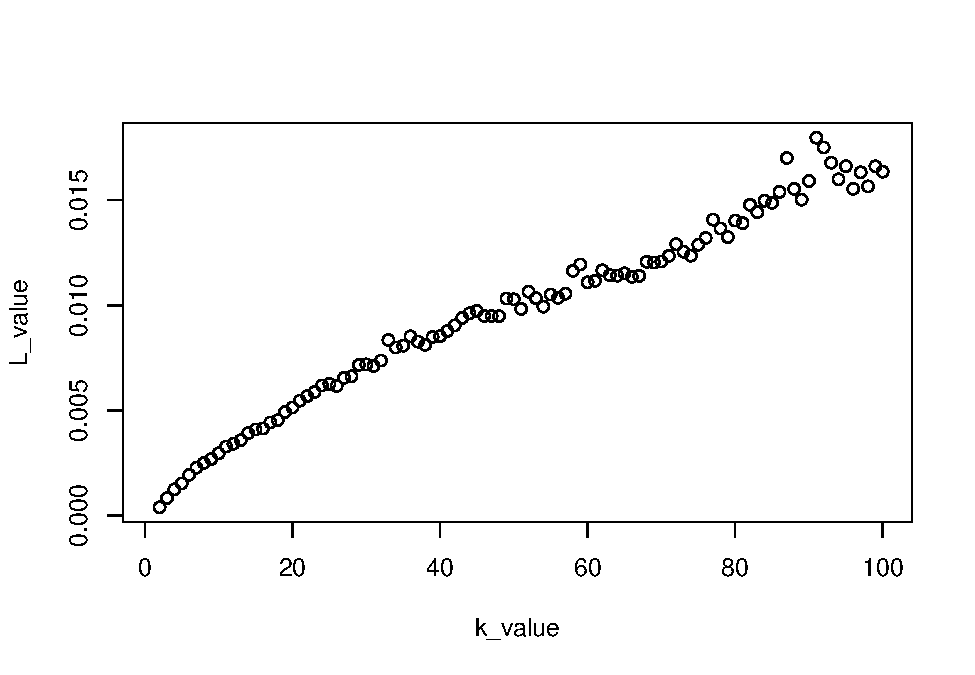
\includegraphics{DP_Second_Laboratory_files/figure-latex/unnamed-chunk-17-1.pdf}

Finally we can observe the correlation between the K and L value
obtained when increasing the value of K.

\end{document}
